\begin{figure}[p]
  \centering
  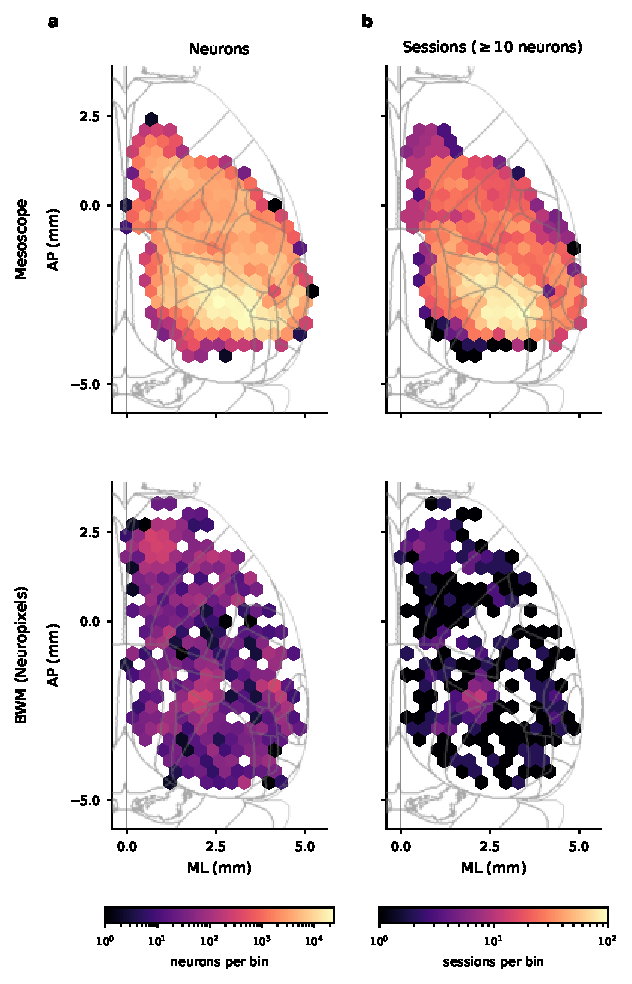
\includegraphics[width=4.32in,height=0.78\textheight,keepaspectratio]{figures/fig2_coverage/dorsal_counts_panels.pdf}
  \caption{Dorsal cortex maps, mesoscope two-photon imaging (top row; deconvolved activity of isocortex neurons, canonical sessions) vs Brain Wide Map Neuropixels recordings (bottom row; good isocortex units, 2023 release). Each neuron is assigned to a hexagonal bin (0.4\,mm vertex to vertex) by its medio-lateral (ML) and antero-posterior (AP) Allen CCF position relative to bregma; both hemispheres are folded onto the right one (ML $\to$ $|$ML$|$). Grey lines: Allen top-view region boundaries. Trials: choice made and reaction time 0.08--2\,s (BWM criteria). Colour scales are shared between the two rows. \textbf{a} Total number of isocortex neurons recorded in each spatial bin; mesoscope (top; 1,080,309 neurons, 153 sessions) and BWM (bottom; 13,002 good units, 288 sessions). \textbf{b} Number of sessions contributing at least 10 neurons to each bin.}
  \label{fig:fig2_coverage}
\end{figure}
